\documentclass[11pt,letterpaper]{article}
\usepackage[lmargin=1in,rmargin=1in,tmargin=1in,bmargin=1in]{geometry}
\usepackage{../style/homework}
\setbool{quotetype}{true} % True: Side; False: Under
\setbool{hideans}{true} % Student: True; Instructor: False

% -------------------
% Content
% -------------------
\begin{document}

\homework{16: Due 04/10}{Mankind was born on Earth\dots it was never meant to die here.}{Joseph Cooper, Interstellar}

% Problem 1
\problem{10} Sketch the function $f(x)= (x + 6)^2 - 5$.
	\[
	\fbox{
	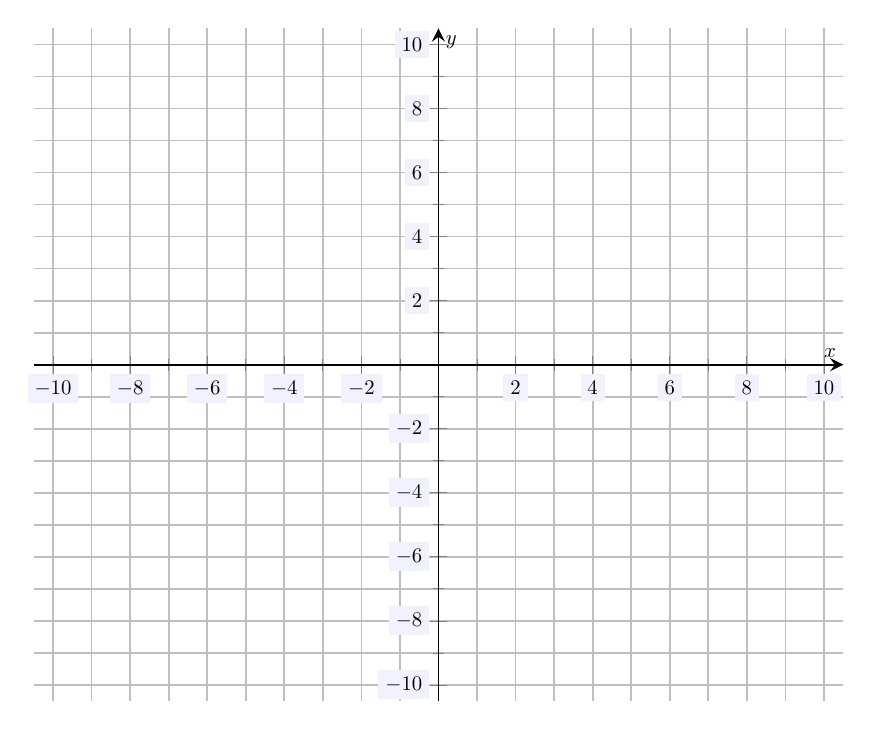
\begin{tikzpicture}[scale=1.5,every node/.style={scale=0.5}]
	\begin{axis}[
	grid=both,
	axis lines=middle,
	ticklabel style={fill=blue!5!white},
	xmin= -10.5, xmax=10.5,
	ymin= -10.5, ymax=10.5,
	xtick={-10,-8,-6,-4,-2,0,2,4,6,8,10},
	ytick={-10,-8,-6,-4,-2,0,2,4,6,8,10},
	minor tick = {-10,-9,...,10},
	xlabel=\(x\),ylabel=\(y\),
	]
	\end{axis}
	\end{tikzpicture}
	}
	\]



\newpage



% Problem 2
\problem{10} Find the equation of the quadratic function shown below. Be sure to fully justify why your answer is correct.
	\[
	\fbox{
	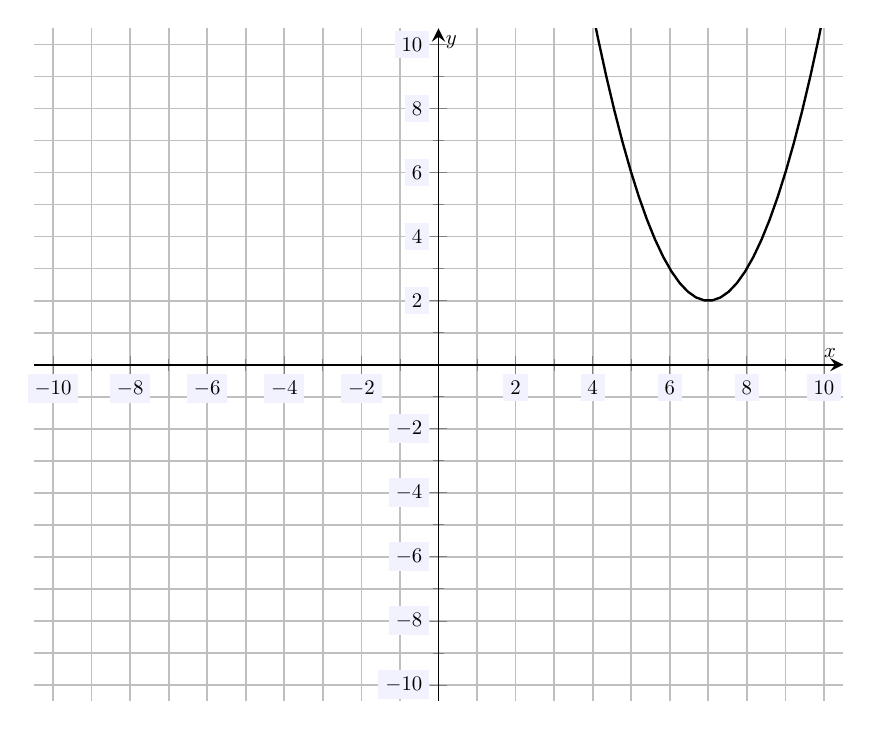
\begin{tikzpicture}[scale=1.5,every node/.style={scale=0.5}]
	\begin{axis}[
	grid=both,
	axis lines=middle,
	ticklabel style={fill=blue!5!white},
	xmin= -10.5, xmax=10.5,
	ymin= -10.5, ymax=10.5,
	xtick={-10,-8,-6,-4,-2,0,2,4,6,8,10},
	ytick={-10,-8,-6,-4,-2,0,2,4,6,8,10},
	minor tick = {-10,-9,...,10},
	xlabel=\(x\),ylabel=\(y\),
	]
	\addplot[line width= 0.02cm,samples=100,domain= -10.5:10.5] ({x},{(x - 7)^2 + 2});
	\end{axis}
	\end{tikzpicture}
	}
	\]



\newpage



% Problem 3
\problem{10} Consider the quadratic function $f(x)= -x^2 - 4x + 12$.
	\begin{enumerate}[(a)]
	\item Find $a, b, c$ for this quadratic function.
	\item Does $f(x)$ open upwards or downwards? Explain.
	\item Is this quadratic function convex or concave? Explain. 
	\item Find the minimum value of $f(x)$, if it exists. If it does not exist, explain why.  
	\item Find the maximum value of $f(x)$, if it exists. If it does not exist, explain why. 
	\end{enumerate}



\newpage



% Problem 4
\problem{10} Consider the quadratic function $f(x)= (x + 3)^2 - 10$.
	\begin{enumerate}[(a)]
	\item Find $a, b, c$ for this quadratic function.
	\item Does $f(x)$ open upwards or downwards? Explain.
	\item Is this quadratic function convex or concave? Explain. 
	\item Find the minimum value of $f(x)$, if it exists. If it does not exist, explain why.  
	\item Find the maximum value of $f(x)$, if it exists. If it does not exist, explain why. 
	\end{enumerate}


\end{document}